
%%%%%%%%%%%%%%%%%%%%%%%%%%%%%%%%%%%%%%%%%%%%%%%%%%%%%%%%%%%%%%%%%%%%%%%%%%%%%
%%%%% Basic C++ %%%%%%%%%%%%%%%%%%%%%%%%%%%%%%%%%%%%%%%%%%%%%%%%%%%%%%%%%%%%%
%%%%%%%%%%%%%%%%%%%%%%%%%%%%%%%%%%%%%%%%%%%%%%%%%%%%%%%%%%%%%%%%%%%%%%%%%%%%%
\begin{frame}
\pointedsl{
	Basics
}
\end{frame}

%
% Content:
% 1. Variables (declaration, assignment, operations)
% 2. Types (list: char, short, int, float, double, bool, void; typedef)
% 3. Expressions (unary, binary, arithmetic, comparator, bitwise)
% 4. Conditions (if, else if, else)
% 5. Loops (for, while, do while)
% 6. Arrays
% 7. Functions (declaration, definition, signature /!\ types -> diff fun)

%%%%%%%%%%%%%%%%%%%%%%%%%%%%%%%%%%%%%%%%%%%%%%%%%%%%%%%%%%%%%%%%%%%%%%%%%%%%%
\lstset{numbers=none}
\begin{frame}[fragile]
\frametitle{Variables}
\begin{lstlisting}
int x; // declare a variable of type "int"
x = 7; // assign a value to "x"
int y = 2; // declare and assign 2 to "y"
y = y * 2; // multiply by 2, then reassign
y *= 2; // shorter version of above
int z = (y - 2) * x; // z equals 42
\end{lstlisting}
\misc{
	\textbf{Variables} are used to store data.
	
	Each variable posesses 
	\begin{itemize}
		\item a \emph{name} (\ctext{x}, \ctext{y}, \ctext{z})
		\item a \emph{type} (\ctext{int} for integer)
	\end{itemize}
	that enable the program to locate and interpret the data.
}
\end{frame}

%%%%%%%%%%%%%%%%%%%%%%%%%%%%%%%%%%%%%%%%%%%%%%%%%%%%%%%%%%%%%%%%%%%%%%%%%%%%%
\begin{frame}[fragile]
\frametitle{Variable types}
\begin{center}
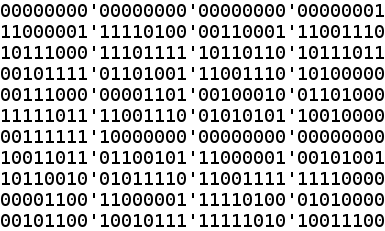
\includegraphics[width=0.6\textwidth]{figures/bits_black}
\end{center}
\misc{
	Computer data consists of sequences of '0' and '1' (bits).
	
	The type of a variable provides an interpretation of the data sequence. Without a type, the bits may mean anything.
}
\end{frame}

\begin{frame}[fragile]
\frametitle{Variable types}
\misc{
	Fundamental types include:
	\begin{itemize}
		\item \textbf{Integer types}: \ctext{char}${}^{(*)}$, \ctext{short}, \ctext{int}, \ctext{long} \\(each in \ctext{signed} or \ctext{unsigned} version)
		\item \textbf{Floating point types}: \ctext{float}, \ctext{double}
		\item \textbf{Boolean type:} \ctext{bool}
	\end{itemize}
	Each has a specific \emph{size} in memory and can only represent a limited amount of distinct values (the type \emph{range}).
}
\begin{lstlisting}
unsigned int n = 1; bool f = true;
char c = 'a'; double pi = 3.14159;
\end{lstlisting}
\end{frame}

\begin{frame}[fragile]
\frametitle{Variable types}
\begin{center}
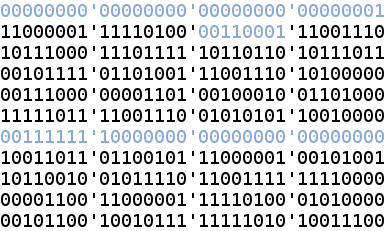
\includegraphics[width=0.6\textwidth]{figures/bits}
\end{center}
\lstset{
	xleftmargin=3cm
}
\begin{lstlisting}
int i = 1;
char c = '1';
float f = 1.0f;
\end{lstlisting}
\end{frame}

%%%%%%%%%%%%%%%%%%%%%%%%%%%%%%%%%%%%%%%%%%%%%%%%%%%%%%%%%%%%%%%%%%%%%%%%%%%%%
\begin{frame}[fragile]
\frametitle{Operators}
\misc{
	Each type has a set of (unary and binary) \textbf{operators}.
}
\begin{columns}[c]
  \begin{column}{0.5\textwidth}
\begin{lstlisting}
// arithmetic
// for numbers
+ - * / %
// bitwise
// for integers
& | ^ ~ >> <<
// incr- decrement
// for integers
++ --
\end{lstlisting}
  \end{column}
  \begin{column}{0.5\textwidth}
\begin{lstlisting}
// comparison
// producing bool
== != < <= > >=
// logical
// for bool
! || &&
// accessors
. :: * & ->
, [] ()
\end{lstlisting}
  \end{column}
\end{columns}
\end{frame}

\begin{frame}[fragile]
\frametitle{Operators}
\misc{
	When creating new types, one can overload the operator's behavior.
}
\begin{lstlisting}
std::cout << "Hello world!\n";
int input_number;
std::cin >> input_number;
\end{lstlisting}
\misc{
	For example, \ctext{Stream} objects use \ctext{<<} and \ctext{>>} as
	output and input operators.
}
\end{frame}

%%%%%%%%%%%%%%%%%%%%%%%%%%%%%%%%%%%%%%%%%%%%%%%%%%%%%%%%%%%%%%%%%%%%%%%%%%%%%
\begin{frame}[fragile]
\frametitle{Sequential flow}
\misc{
	The simplest programs are \textbf{sequential}: they execute a sequence of statements in the order they are written.
}
\end{frame}

\begin{frame}[fragile]
\frametitle{Sequential flow}
\begin{columns}[c]
  \begin{column}{0.5\textwidth}
  \hfill
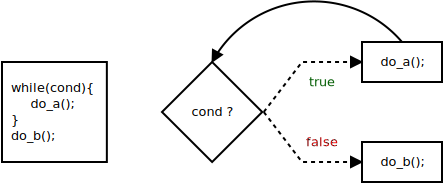
\includegraphics[scale=0.5]{figures/flow}
  \end{column}
  \begin{column}{0.5\textwidth}
\begin{lstlisting}
statement_1;
statement_2;
...
statement_N;

// Question:
// How to act
// according to
// the input?
\end{lstlisting}
  \end{column}
\end{columns}
\end{frame}

\begin{frame}[fragile]
\frametitle{Sequential flow}
\misc{
	The two main ways of breaking this sequential behavior are
	\begin{enumerate}
		\item \textbf{conditions} that execute statements only if a condition is met (or not) and
		\item \textbf{loops} that repeatedly execute statements until a specific state is reached (modeled as a condition).
	\end{enumerate}
}
\end{frame}

%%%%%%%%%%%%%%%%%%%%%%%%%%%%%%%%%%%%%%%%%%%%%%%%%%%%%%%%%%%%%%%%%%%%%%%%%%%%%
\begin{frame}[fragile]
\frametitle{Conditional flow}
\begin{columns}[c]
  \begin{column}{0.5\textwidth}
  \hfill
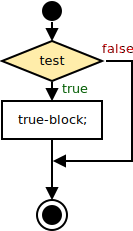
\includegraphics[scale=0.5]{figures/flow-ifthen}
  \end{column}
  \begin{column}{0.5\textwidth}
\begin{lstlisting}
if( test ){
  true_block;
}

// Question:
// Special action
// when the test
// fails?
\end{lstlisting}
  \end{column}
\end{columns}
\end{frame}

\begin{frame}[fragile]
\frametitle{Conditional flow}
\begin{columns}[c]
  \begin{column}{0.5\textwidth}
  \hfill
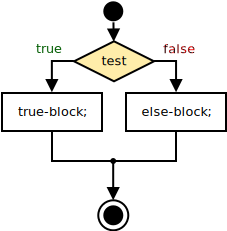
\includegraphics[scale=0.5]{figures/flow-ifelse}
  \end{column}
  \begin{column}{0.5\textwidth}
\begin{lstlisting}
if( test ){
  true_block;
} else {
  else_block;
}

// Note:
// Can be chained
// using
// else if(test)
\end{lstlisting}
  \end{column}
\end{columns}
\end{frame}

%%%%%%%%%%%%%%%%%%%%%%%%%%%%%%%%%%%%%%%%%%%%%%%%%%%%%%%%%%%%%%%%%%%%%%%%%%%%%
\begin{frame}[fragile]
\frametitle{Iterative flow: do-while}
\begin{columns}[c]
  \begin{column}{0.5\textwidth}
  \hfill
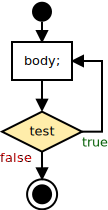
\includegraphics[scale=0.5]{figures/flow-do}
  \end{column}
  \begin{column}{0.5\textwidth}
\begin{lstlisting}
do {
  body;
} while( test );

// Question:
// How to check
// the test
// before body?
\end{lstlisting}
  \end{column}
\end{columns}
\end{frame}

\begin{frame}[fragile]
\frametitle{Iterative flow: while-loop}
\begin{columns}[c]
  \begin{column}{0.5\textwidth}
  \hfill
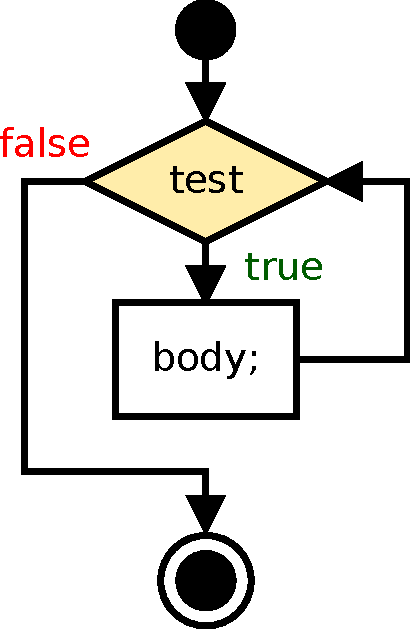
\includegraphics[scale=0.5]{figures/flow-while}
  \end{column}
  \begin{column}{0.5\textwidth}
\begin{lstlisting}
while(test){
  body;
}

// e.g.
while(i > 0){
  ...
  --i;
}
\end{lstlisting}
  \end{column}
\end{columns}
\end{frame}

\begin{frame}[fragile]
\frametitle{Iterative flow: for-loop}
\begin{columns}[c]
  \begin{column}{0.5\textwidth}
  \hfill
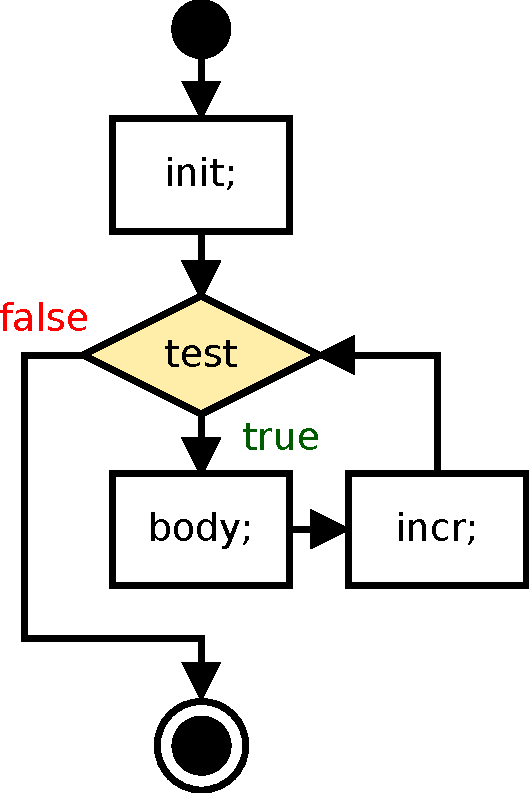
\includegraphics[scale=0.5]{figures/flow-for}
  \end{column}
  \begin{column}{0.5\textwidth}
\begin{lstlisting}
// for (a; b; c){}
for(init;
    test;
    incr){
  body;
}

// e.g.
for(int i = 0;
    i < 5; ++i){
  // loops 5 times
}
\end{lstlisting}
  \end{column}
\end{columns}
\end{frame}

%%%%%%%%%%%%%%%%%%%%%%%%%%%%%%%%%%%%%%%%%%%%%%%%%%%%%%%%%%%%%%%%%%%%%%%%%%%%%
\begin{frame}[fragile]
\frametitle{Loops, variables \& indexing}
\misc{
	Loops are important when processing a lot of similar data.
}
\begin{lstlisting}
int N = 0;
for(int i = 1; i < 100; ++i){
  N += i; // sum from 1 to 100
}
\end{lstlisting}
\misc{
	Here \ctext{N} refers to the same location
	whatever the value of \ctext{i}. What if we
	want a variable that depends on \ctext{i}?
}
\end{frame}

\begin{frame}[fragile]
\frametitle{Arrays}
\begin{columns}[c]
  \begin{column}{0.5\textwidth}
\lstset{numbers=left}
\begin{lstlisting}
int a[3] = { 1, 0 };
a[1] = 42;
// a[2] == 0
\end{lstlisting}
  \end{column}
  \begin{column}{0.5\textwidth}
    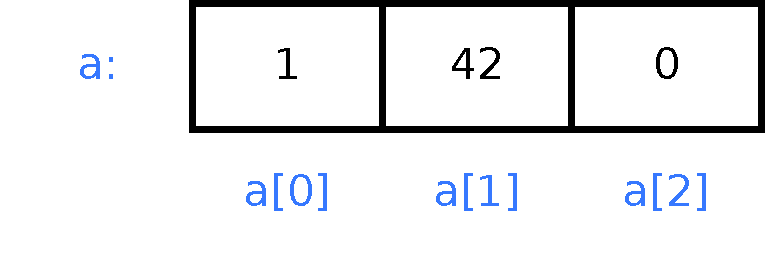
\includegraphics[width=0.95\textwidth]{figures/array0}
  \end{column}
\end{columns}
\misc{
	\emph{Arrays} are continuous blocks of memory that store multiple elements of a same type. They use $0$-based indexing.
	
	They are the storage of choice for multiple instances of a data type.
}
\end{frame}

%%%%%%%%%%%%%%%%%%%%%%%%%%%%%%%%%%%%%%%%%%%%%%%%%%%%%%%%%%%%%%%%%%%%%%%%%%%%%
\begin{frame}[fragile]
\frametitle{Functions}
\misc{
	Functions are pieces of program that can be executed as a whole.
}
\begin{lstlisting}
// How to get sum of integers
// from A to B?
int sum = 0;
for(int i = A; i <= B; ++i)
  sum += i;
  
// and from C to D?
// Copy code again?
\end{lstlisting}
\end{frame}

\begin{frame}[fragile]
\frametitle{Functions}
\begin{lstlisting}
int intSum(int A, int B){
  int sum = 0;
  for(int i = A; i <= B; ++i)
    sum += i;
  return sum;
}
\end{lstlisting}
\misc{
	Here \ctext{intSum} is a function that:
	\begin{itemize}
		\item takes two integer arguments \ctext{A} and \ctext{B}
		\item return the sum of integers between \ctext{A} and \ctext{B}
	\end{itemize}
}
\end{frame}

\begin{frame}[fragile]
\frametitle{Functions}
\begin{lstlisting}
// declare function
// (define it somewhere else)
int intSum(int, int);

// use function
int x = intSum(0, 100);
int y = x + intSum(101, 200);
// y == intSum(0, 200)
\end{lstlisting}
\misc{
	Functions must be \textbf{declared} before being used
	just like variables.
}
\end{frame}

\begin{frame}[fragile]
\frametitle{Functions}
\begin{lstlisting}
// /!\ different functions
int intSum(int, int);
int intSum(float);

// redeclare
int intSum(int x, int y);
// Note: argument names
// are irrelevant
\end{lstlisting}
\misc{
	They can be declared multiple times
	as long as the signature (name + types)
	match.
}
\end{frame}